% In here should add the integral of Mattias hand written notes and corrections
% that David has found to signs and amplitudes

% FIX NOTATION OF \psi -> \Psi for poloidal flux.  \psi is the radial coord = r/R only.
% REMOVE CGS units

\chapter{Tearing modes}

Here are some brief notes that describe how an imposed magnetic island is included in GKW 
(self-consistent tearing modes can occur naturally given correct inputs and thus do not 
require a description of their implementation here). 
The previous version (Refs~\cite{HOR10,HOR10epl}) assumed that the island is always initialised
in the largest poloidal mode.  To have the island in a larger wavevector there are some subtleties to the initialisation.   
For a recent description of the implementation and benchmarks in slab geometry, see 
Zarzoso et al,. PoP, 2015.

\section{Spectral implementation of magnetic islands in toroidal geometry}
If we initially assume a constant poloidal flux perturbation with a given helicity 
\begin{equation} 
A_\parallel = A_{\parallel0} \exp [ 2 \pi {\rm i} (m s - n \gamma ) ] 
\end{equation} 
where $s$ and $\gamma$ are the poloidal and toroidal angles, respectively.  Introducing the helical coordinate $\zeta = qs - \gamma$ and expanding the safety factor up to first order
\begin{equation} 
q = m / n + \Delta\psi\partial q /\partial\psi
\end{equation} 
in the centre of the box (i.e. the mode is resonant at this position). We need to transform this
representation to the ($\psi, \zeta, s)$ coordinate system which gives,
\begin{equation} 
A_\parallel = A_{\parallel0} \exp [ 2 \pi {\rm i} ( n \zeta - {\partial q \over \partial \psi} n s \Delta\psi ) ] 
\end{equation} 
From which it directly follows that 
\begin{equation} 
k_\zeta = 2 \pi n \rho_* 
\end{equation}
is the toroidal mode of the island.  However for generality we assume that this may not be the largest wavelength within the domain, this is $k_\zeta^{min} = 2\pi\rho_*$.

In the helical field line co-ordinate system the x-points only appear in the $\zeta$ direction.  In the toroidal and poloidal angles, x-points appear in both.  
From the periodicity constraint connected with the parallel boundary conditions it follows that the radial wavevectors are given by
\begin{equation} 
 k_\psi = (p/i_k) k_\zeta {\partial q \over \partial \psi} = (p/i_k) 2 \pi \rho_* {\partial q \over \partial \psi} 
\end{equation} 
where $p$ is a set of integers in the range $[-N_x/2, N_x/2]$ and $i_k$ is the parameter that determines the radial mode spacing.  
From $p = 1$ one directly obtains the radial size of the box 
\begin{equation} 
\psi = \biggl [ - { i_k \over 2 \partial q / \partial \psi} , {i_k \over 2 \partial q / \partial \psi} \biggr ] \cdot {1 \over k_\zeta^{min}} 
\end{equation}

The Fourier amplitudes of the different radial modes then can be calculated by integrating over 
the radial domain 
\begin{align}
\hat{A}(k_\psi, k_\zeta, s) &=& A_{\parallel0} \exp{(i\ n k_\zeta^{min}\zeta)}\int {\rm d} \Delta\psi \exp{\biggl [i\Delta\psi( k_\psi + n s k_\zeta^{min} dq/d\psi)   \biggr ]} \nonumber\\
&=& {A_{\parallel0} i_k \over \pi n \partial q / \partial \psi} {\sin [ \pi (n i_k s + p) ] \over n i_k s + p}  \nonumber\\
&=& C{i_k \over n} {\sin [ \pi s^\circ ] \over s^\circ} 
\end{align}
where we have used the ballooning angle $s^\circ = n i_k s + p$ in the last step and $n$ is the poloidal wave mode (determined by the input parameter \name{isl_mode}).

One point to note at this point is that this perturbation is not periodic in the radial domain of GKW for all values of $s$.  This manifests itself as a discontinuity in the parallel vector potential at the radial edge of the computational domain.  A solution to this problem is to relax the constant flux approximation and therefore write the perturbation as,
\begin{equation} 
A_\parallel = C{i_k \over n} \exp{i k_{\zeta}\zeta}\sum_{p=N_x/2}^{N_x/2} A^{p}(s)\exp{i pk_{\psi}\Delta\psi}
\end{equation}  
Where $A^{p}(s)$ includes a damping function.  We have chosen a Gaussian profile to reduce any ringing.  This gives
\begin{equation}
A^{p}(s) = \exp{\left((-(n i_k s + p)^{2}/L_s^{2})\right)}\frac{\sin{\pi(n i_k s + p)}}{(n i_k s + p)}
\end{equation}
Where L is half width of the gaussian envelope.  This approximation leads to a more satisfactory shape for the vector potential, where the value of L can be tuned to that the damping of the small k modes is negligible and the of high k modes sufficiently strongly to prevent the occurance of a jump at the boundary.

Thus the full implemented vector potential has the form,
\begin{equation}
A_{||} = C {i_k \over n} \exp{(i k_{\zeta}\zeta - i\omega t)}\sum_{p=N_x/2}^{N_x/2}\exp{\left(-\frac{(n i_k s + p)^2}{L_s^2}\right)}\frac{\sin{\pi((n i_k s + p))}}{(n i_k s + p)}\exp{(i p k_{\psi}\Delta\psi)}
\end{equation}
where $\omega$ is the poloidal rotation frequency of the island.  Note that only a single binormal mode is used.  The island half-width is defined in dimensional units (Wesson) as 
\begin{equation}
W = 2\sqrt{\frac{rq \tilde B_{r}}{m B_p (dq/dr)}} = 2\sqrt{\frac{r \tilde A_\parallel}{B_p {\hat s}}} = 2\sqrt{\frac{q R \tilde A_\parallel}{B_t {\hat s}}}
\end{equation}
where $B_p$ is the poloidal component of the background magnetic field\footnote{The correspondance with the literature on the sheared slab by Smolyakov and others is as follows: They have $W^2 = 4 L_s A_{\parallel} / B_0$, but $\psi$ is the vector potential in their notation.  The toroidal result used in GKW can be obtained by inserting $1/L_s = (1/q)(dq/dr)$, and $B_0 = B_p$.}.  The island width determines the amplitude of the island perturbation:  The factor $dq/dr = q {\hat s} / r$ is obtained from the magnetic shear and $m$ is the poloidal mode number.  Using the fact that the peturbed radial magnetic field is prescribed as $\tilde{B}_{r}= m\tilde{\Psi} /rR$, and that for the $s-\alpha$ model equilibrium the perturbed magnetic flux is given by $\tilde{\Psi} = R\tilde{A}_{\parallel 0}$, and $q=r B_t / R B_p$, the amplitude of the island vector potential (now in GKW normalised units) is given by
\begin{equation}
\tilde{A}_{\parallel0N} = {W_N^2 B_{tN} {\hat s} \over 4 q R_N}, \qquad  C = {W_N^2 B_{tN} \epsilon \over 4 \pi q^2 R_N}.
\label{aparamp}
\end{equation} 
where $B_t^N$ is taken at the low field side in order to define the island width at the same location, and $W = W_N \rho_{\rm ref}$. Note that the amplitude of C given in equation \ref{aparamp} is divided by 2, due to the form of the Fourier representation described in Sec. \ref{sec:spectral}.  % HOW IS C OBTAINED - THE BOX SIZE with dq/dpsi = shat q /eps - eqn 5.6 enters   ?
%the fact that
%the island is actually a perturbation in real space (not in Fourier space), which must be of the form
%$\cos\left[2\pi\left(ms-n\gamma\right)\right]$.


\begin{figure}
\begin{center}
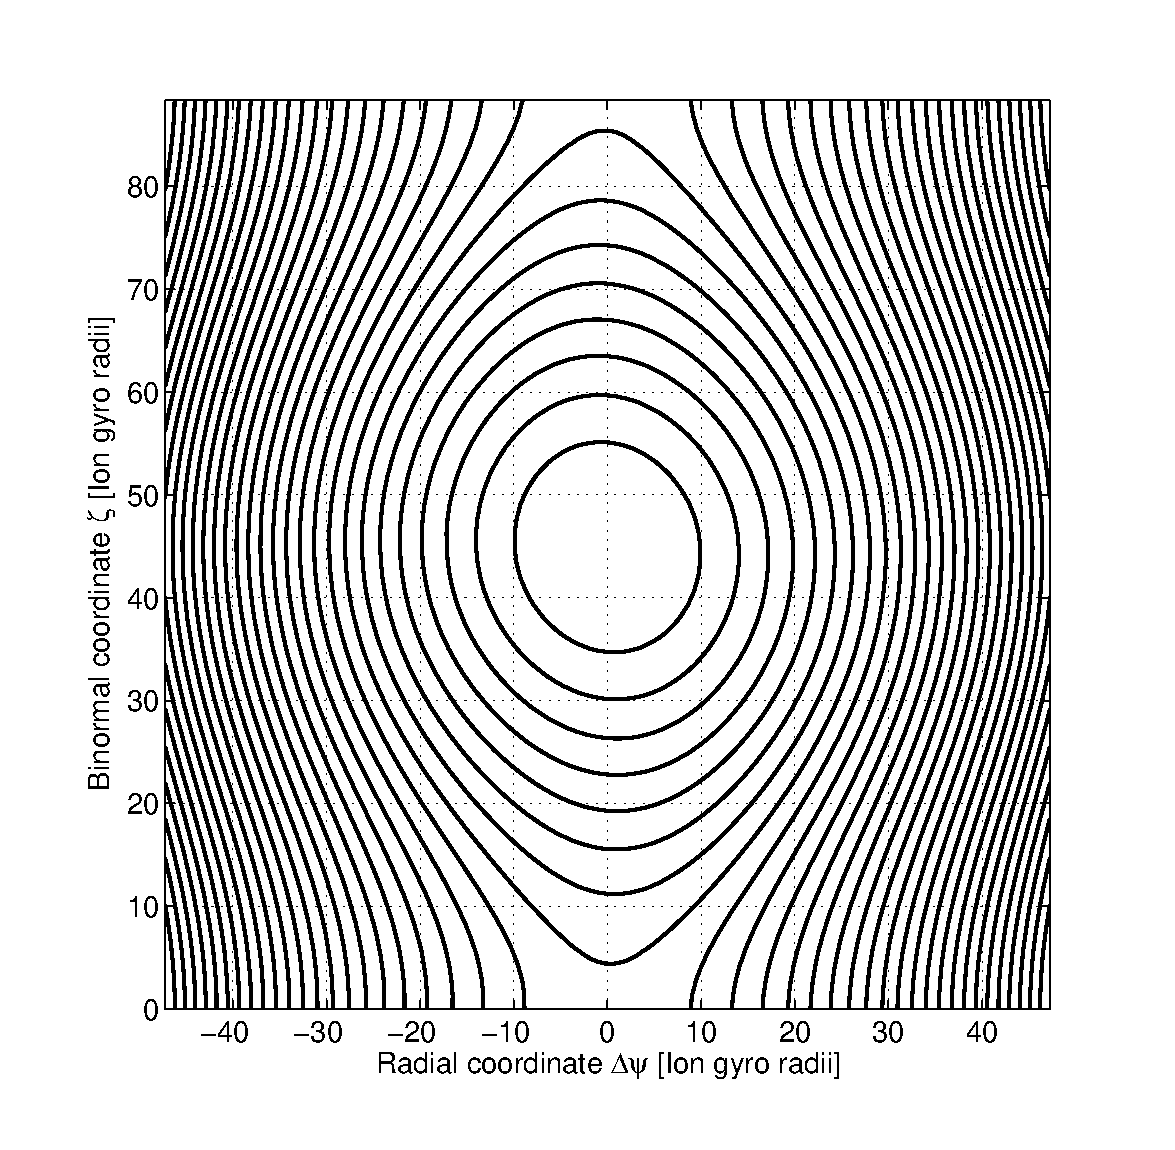
\includegraphics[width=0.3\textwidth]{MagIslGeom.eps}
\caption{Magnetic Island Geometry for an island with a half width of 30 ion gyro-radii}
\label{islandgeom}
\end{center}
\end{figure}

To run GKW with a magnetic island present the following options must be used:  Firstly, the code must be set to run electro-magnetically by setting \name{nlapar=.true.}.  In the \name{SPCGENERAL} namelist, \name{tearingmode} must be set to {\it .true.}, which adds the magnetic island as a perturbation of the equilibrium field.  The half width of the island is determined by the input parameter \name{wstar} which is the island width normalised to $\rho_{ref}$ (usually the ion gyro-radius).  A point of note is that this island width can not exceed (and should be smaller than) the radial extent of the computational box due to the periodicity constraints of a pseudo-spectral code. The rotation frequency of the island ($\omega$) is set by the parameter \name{isl\_rot\_freq}, normalised as other frequencies in the code BUT with opposite sign (positive is in the $\nabla \zeta$ direction, which is the electron grad-B drift direction when $s_j = 1$ and rln > 0.  By default the island is placed in the smallest non-zero poloidal wavevector (\name{isl\_mode=2}), however this can be changed by setting \name{isl\_mode} to another integer (e.g. \name{isl\_mode=3} will give 2 islands within the domain as the zero mode is always the first mode).

We recommend initialising the distribution function with \name{finit='zero'} as the island itself will seed the turbulence, and this gives faster convergence compared to non-zero distribution function initialisations.  When plotting XY profile outputs, setting {\it lisl_follow} in the \name{DIAGNOSTIC} namelist will follow the magnetic island so that the O-point is always in the centre of the box.  We do not recommend using the options to initialise the island after the turbulence, as growing the island too quickly drives a unphysical and large zonal flow, which initally supresses the turbulence and then takes a long time to decay.

\begin{small}
\begin{verbatim}
 &SPCGENERAL
 beta = 0.0001,  ! not used
 tearingmode=.true.,  wstar = 5.0,  finit = 'zero',  adiabatic_electrons = .false.
 Ls = 2.0,  isl_mode = 2, isl_rot_freq = 0.1   
 /
\end{verbatim}
\end{small}

\section{Spectral implementation of islands in 2D sheared slab geometry}

An alternative way to deal with 2D islands is also implemented, in which
parallel dynamics are projected into the $y$ direction, 
as is usually done in slab analytics.  This allows GKW islands to be compared
directly with analytical results in the slab.   Whilst this setup is intended for use with the slab geometry, 
it might also be applicable for a LFS toroidal case.
The island amplitude is decoupled from geometric magnetic shear, and 
a new parameter, \name{isl\_shear} is used in determing the island width.
To use this option the geometric shear \name{shat} is set to 0 (which
means reducing the coordinate system to purely Cartesian) and the code is
run with a single s point and without parallel dynamics 
(a limit in which the geometrical magnetic shear plays no role).
This also implies that the minimum $k_x$ and $k_y$ now can be set completely
independently, but they are chosen to be the same (to give a square box).

The perturbed $A_\parallel$ in this case then also contains the part of the island that
normally comes from the background magnetic field (in the 2D case the background B
plays no role in the geometry and theoretically only enters via the Larmor
radius). The slab geometry is defined in this case through a Cartesian set of
coordinates, $x$,$y$ and $z$, where $z$, the direction of the guide magnetic
field, is meant to be a symmetry coordinate for the whole system,
i.e. $\partial/\partial z = 0$, accordingly to the existing dedicated literature. 
The total magnetic field in this case reads
\begin{equation}
{\bf B} = B_z \nabla z -\nabla \psi \times \nabla z,
\end{equation}
with 
\begin{equation}
\psi = -\frac{i_s x^2}{2}B_z+\tilde{\psi}\cos( k_y y),
\label{psiisl}
\end{equation}
where $B_z$ is a constant and where  $i_s$ corresponds to \name{isl\_shear},
the (inverse of the) scale of variation of $B_y$, which plays a role analogous
to the magnetic shear in toroidal geometry. The $y$-dependent term represents
the island.  The amplitude $\tilde{\psi}$, assumed to be constant as a
consequence of the well-known ``constant-$\psi$ approximation'', is  linked to the island width $w$ through the relation
\begin{equation}
w^2=\frac{4 \tilde{\psi}}{i_s B_z}.
\end{equation}

In the 3D case, only the latter ``island''-part of $\psi$ is imposed as a
perturbation, entering the gyrokinetic equation through $v_\chi$ in the nonlinear term. 
In this 2D case, in constrast, we consider a shearless slab, with equilibrium 
\begin{equation}
{\bf B}= B_z \nabla z
\end{equation}
(constant) and we include the whole $\psi$ of Eq. \ref{psiisl}
as a perturbation. In Fourier space this extra island component
(additional to the usual part in the island $k_y$ mode)
is applied in the $k_y=0$ mode, and has the form 
\begin{equation}
A_\parallel^+(p) =  {4 (-1)^p i_s \over {\bar k}_x(p)^2 } \exp(-(p/Ls)^2)
\end{equation} 
where $p$ is again the radial mode number, and an exponential damping has again 
be added to the exact Fourier transformed quantity. The overbar on ${\bar k}_x$
represents the modes in the code, to distinguish them from the island wavenumbers $k_x$ and $k_y$
used above.  While it is apparent that $\psi$ is periodic on $y$, the
quadratic dependence on $x$ cannot be exactly reproduced in Fourier space, as
its derivative is not the same on the two boundaries. Thus, analogously to
the toroidal case, we again employ the exponential damping for the high $k_x$ modes in
order to remove boundary discontinuities.  This approximation has the effect of creating a second
magnetic island at the boundary which in full 3D geometry is obscured by parallel coupling, ballooning
and curvature. The effect of this boundary island can be minimised by 
choosing an appropriate combination of the parameters box size, shear, island width, damping length
(which differ in slab and torodial geometry) but it can never be completely eliminated.

In the 2D case, there is however an additional island option, to add \textit{two}
identical islands radially with perfect periodicity.  This option is activated
when \name{shat} = 0 and \name{isl\_shear} $> 0$ by selecting a
negative \name{wstar}. By choosing this option,  $\psi$ is
approximated by 
\begin{equation}
\psi = {\hat C}\cos{k_x x}+\tilde{\psi}\cos{k_y y},
\end{equation}
where $\hat{C}= \pi B_z i_s/ k_x^2$ is a constant chosen in order to have the
same amplitude as the other case for $B_y= \partial \psi/\partial$ at the edge
of the box. In this case, the additional nonzero component only appears in the $k_y=0$, $p= -1,1$ modes
with value $A_\parallel^+ = \pi i_s / k_x^2$.  The sinusoidal dependence can of course be implemented without any
approximation, or artificial damping, leading therefore to no parasitic boundary island
formation. However, the presence of both a maximum and a minimum in $x$
corresponds to the presence of two identical islands with $\pi/2$-shift in the
$y$-direction. By carefully choosing the box width, one is able to reduce the
mutual interaction of the two islands. 

Summarizing, for slab geometry GKW  has three options for islands:
\begin{itemize}
\item To run with shat $>$ 0 in 3D, which is expensive (and where
discontinuities at the boundary create numerical problems) and which does not
reproduce the boundary condition $\partial / \partial z =0$ used in many analytic models.
\item To run with shat = 0 and wstar $>$ 0. These are 2D runs, much faster, but which still
employ the artificial damping on high- ${\bar k}_x$ modes, and therefore require
specific attention to the discontinuity at the boundary, as in the full 3D cases.
\item To run with shat = 0 and wstar $<$  0. These are 2D runs, with no
artificial damping, but which contain two identical out of phase magnetic
islands at two radial locations.
\end{itemize}

Example 2D setup:
\begin{small}
\begin{verbatim}
 &GRIDSIZE
 NX = 167,  N_mu_grid = 8,  n_vpar_grid = 12, number_of_species = 2,
 N_s_grid = 1,  NMOD = 20,  nperiod = 1,
 /
 &MODE
 mode_box = .true., krhomax = 0.45, ikxspace = 1,
 /
 &GEOM
 GEOM_TYPE = 'slab_periodic', SHAT = 0.0,  Q = 1.0, EPS = 1.0,
 /
 &SPCGENERAL
 finit = 'zero',  tearingmode=.true.,
 wstar = 10.0, isl_rot_freq = -0.02,
 adiabatic_electrons = .false.
 ls=8.0, isl_shear = 0.1
\end{verbatim}
\end{small}

\section{Nonspectral implementation of a magnetic island}

If the radial direction is not treated in Fourier space, the implementation is much more direct, since we need only to introduce at $t=0$ the term
\begin{equation}
A_\parallel = A_{\parallel 0}\cos\left(2 \pi {\rm i} (m s - n \gamma )\right)
\end{equation}
which can be expressed by
\begin{equation}
A_\parallel = {1\over 2}A_{\parallel 0}\left[e^{i2\pi n\zeta}\left(\cos{\partial q \over \partial \psi} n s \Delta\psi - i\sin{\partial q \over \partial \psi} n s \Delta\psi\right)
+ e^{-i2\pi n\zeta}\left(\cos{\partial q \over \partial \psi} n s \Delta\psi + i\sin{\partial q \over \partial \psi} n s \Delta\psi\right)\right]
\end{equation}

In the binormal direction we initialise only one mode, namely $e^{i2\pi n\zeta}$ and assume the existence of the other mode in other to get a real quantity once the inverse Fourier transform is performed. Therefore,
 we need to implement only the potential
 \begin{equation}
A_{\parallel,+} = {1\over 2}A_{\parallel 0}\left(\cos{\partial q \over \partial \psi} n s \Delta\psi - i\sin{\partial q \over \partial \psi} n s \Delta\psi\right)
\end{equation}

In order to decouple the island from the boundary of the simulation box, we multiply the previous potential by a radial envelope having the explicit expression
\begin{equation}
A_r\left(\Delta\psi\right) = {1\over 4}\left(1+\tanh\left({\Delta\psi+\Delta\psi_0\over \delta\psi_0}\right)\right)\left(1-\tanh\left({\Delta\psi-\Delta\psi_0\over \delta\psi_0}\right)\right)
\end{equation}
where $\Delta\psi_0$ and $\delta\psi_0$ are defined in the tearingmode namelist of the input file of GKW by the variables \File{psi_0} and \File{delta_psi_0}, respectively.

In a 2D sheared slab geometry, the previous implementation reduces to
\begin{equation}
A_\parallel = {1\over 2}A_{\parallel 0}A_r\left(\Delta\psi\right)
\end{equation}
and the background magnetic shear is introduced together with this perturbation by means of the mode $\kappa_\zeta=0$. Therefore, the total parallel vector potential reads in 2D sheared slab geometry
\begin{equation}
A_\parallel = {B_zi_s\over 2}\left[\Delta\psi^2-\left(L_x/2\right)^2\right]+{1\over 2}A_{\parallel 0}A_r\left(\Delta\psi\right)e^{i2\pi n\zeta}
\end{equation}
where the additional term ${B_zi_s\over 2}\left(L_x/2\right)^2$ is introduced to impose a vanishing potential at the boundary in the nonspectral version. We therefore need to introduce the term ${B_zi_s\over 2}\left[\Delta\psi^2-\left(L_x/2\right)^2\right]$ in the $\kappa_\zeta=0$ component and the term ${1\over 2}A_{\parallel 0}A_r\left(\Delta\psi\right)$ in the $\kappa_\zeta = \kappa_{\rm isl}$ component.

\section{Reconstruction of flux tube radial profiles \label{profiles} and profile flattening in GKW}

The benchmark of the magnetic islands implementation includes the flattening of the density and pressure profiles. The equilbrium profiles are linear with respect to the radial coordinate and are present in the source terms.  Since we are solving the gyrokinetic equation for the perturbed part of the distribution function, the solution should respond to the source terms due to the background. In particular, the magnetic island should give a perturbation that cancels the background out inside the separatrix. Note that runs must be non-linear for the correct level of flattening to be obtained. To reconstruct the radial profiles the XY diagnostics must enabled in the diagnostics namelist.

% \begin{verbatim}
% &DIAGNOSTIC
%  lisl_follow = .false.,
%  lphi_diagnostics = .true.,
%  xy_phi = .true.,
%  xy_apar = .true.,
%  xy_fluxes = .true.,
%  xy_fluxes_em = .true.,
%  xy_dens = .true.
%  xy_current = .true.,
%  xy_temp = .true.,
%  / 
% \end{verbatim}

\subsection{Density profiles}

The files named \File{den0\#_000*_*} hold the normalised XY perturbed density data ($\tilde{n}_{N,s}$) for each large time step. The background density profile can be reconstructed by using the local radial cordinate $x_r = \psi / \rho_* = r / \rho_{\rm ref}$ which is written in the file named \name{xphi} (with the same dimensions as the XY slices) and the input parameter \name{RLN_s} = $-(1/n_{R_0,s}) {\partial n_{R_0,s} \over \partial \psi}$. The total density of species $s$ is $n_s = n_{s,\rm eq} + \tilde{n}_s$, where $n_{s,\rm eq} = n_{R_0,s}\left(1-{r-r_0\over L_{n,s}}\right)$ is the global density of the Maxwellian equilibrium written in the local limit, i.e. $n_{R_0,s}$ at the resonant position $r_0$ plus the linear variation due to the gradient at that position. Note that in the expression of $n_{s,\rm eq}$, the quantity $n_{R_0,s}$ does not exhibit any radial dependence since it is considered in the local limit. The perturbed density of species $s$ is

\begin{equation}
\tilde{n}_s = \int_{\mathbb R^3} d^3\mathbf{v}\delta f_s = \rho_*n_{R_0,s}\int_{\mathbb R^3} d^3\mathbf{v}_{N,s}\delta f_{N,s} = \rho_*n_{R_0,s}\tilde{n}_{N,s}
\end{equation}

Therefore, the total density for species $s$ reads

\begin{equation}
n_s = n_{R_0,s}\left(1-{r-r_0\over L_{n,s}}\right) + \rho_*n_{R_0,s}\tilde{n}_{N,s} = n_{R_0,s}\left(1 - {\left(x_r-x_{r0}\right)\rho_{\rm ref}\over {L_{n,s}}}\right) + \rho_*n_{R_0,s}\tilde{n}_{N,s}
\end{equation}

We can now normalise the density for species $s$ as $n_{N,s} = n_s / n_{R_0,s}$

\begin{equation}
n_{N,s} = \left(1 - {\left(x_r-x_{r0}\right)\rho_{\rm ref}\over {L_{n,s}}}\right) + \rho_*\tilde{n}_{N,s}
\end{equation}
and define the change in the density for species $s$ as $\Delta n_{N,s} = n_{N,s} - 1$

\begin{equation}
 \Delta n_{N,s} = - \left(x_r-x_{r0}\right){\rho_{\rm ref}R_{\rm ref}\over {L_{n,s}R_{\rm ref}}} + \rho_*\tilde{n}_{N,s}  =  - \rho_* \left(x_r-x_{r0}\right) {R_{\rm ref}\over L_{n,s}} + \rho_*\tilde{n}_{N,s}
\end{equation}
or alternatively
\begin{equation}
{\Delta n_{N,s} \over \rho_*} = \tilde{n}_{N,s} - {R_{\rm ref} \over L_{n,s}} \left(x_r-x_{r0}\right)
\end{equation}
and the total density gradient (background plus perturbed density) can be computed as
\begin{equation}
{R_{\rm ref} \over L_{n_{\rm eq}+\tilde{n}}}  =  -{1 \over n_{R_0,s}} {\partial (n_{s,\rm eq}+\tilde{n}_s) \over \partial \psi} = 
 -{\partial \tilde{n}_{N,s} \over \partial x_r} + {R_{\rm ref} \over L_{n,s}}.
\end{equation}

%PREVIOUS VERSION needs a factor rho_* to get to a normalised total density (i.e. it has the normalisation of delta f, not F_M)
%\begin{equation}
%n({\Delta\psi}) = \tilde{n} - RLn*xphi
%\end{equation}

\subsection{Pressure profiles}
To obtain the pressure profiles we need to use the files \File{ene0\#_000*_*}, which hold the normalised second moments of the distribution function, namely
\begin{equation}
\tilde E_{N,s} = \int_{\mathbb{R}^3}d^3\mathbf{v}_{N,s}\delta f_{N,s}v_{N,s}^2
\end{equation}

It can be shown that the pressure perturbation is written in terms of this quantity as follows
\begin{equation}
\tilde{p}_s = {1\over 3}m_{\rm ref}v_{th,s}^2\rho_* n_{R_0,s}m_{R,s}\tilde E_{N,s}
\end{equation}

Taking into account the definition of the reference temperature $T_{\rm ref}$, one can write

\begin{equation}
\tilde{p}_s = {2\over 3}\rho_* n_{R_0,s}T_{\rm ref}m_{R,s}v_{R,s}^2\tilde E_{N,s}
\end{equation}

In addition, $m_{R,s}v_{R,s}^2=T_{R,s}$ and $T_s = T_{\rm ref}T_{R,s}$, which leads to
\begin{equation}
\tilde{p}_s = {2\over 3}\rho_* n_{R_0,s}T_s\tilde E_{N,s}
\end{equation}

In the same way as has been done with the density, the total pressure is defined as $p_s = p_{s,\rm eq} + \tilde{p}_s$, where $p_{s,\rm eq} = n_{R_0,s}T_s\left(1-{r-r_0\over L_{n,s}}\right)\left(1-{r-r_0\over L_{T,s}}\right)$. In the local limit we can neglect terms of second order in $\rho_*$ and therefore, the equilibrium pressure profile reads
\begin{equation}
p_{s,\rm eq} \approx n_{R_0,s}T_s\left(1-\rho_*\left(x_r-x_{r0}\right){R_{\rm ref}\over L_{n,s}}-\rho_*\left(x_r-x_{r0}\right){R_{\rm ref}\over L_{T,s}}\right)
\end{equation}

We can now divide by $n_{R_0,s}T_s$ and define the change in the normalized pressure as

\begin{equation}
\Delta p_{N,s} = {2\over 3}\rho_*\tilde E_{N,s}-\rho_*\left(x_r-x_{r0}\right){R_{\rm ref}\over L_{n,s}}-\rho_*\left(x_r-x_{r0}\right){R_{\rm ref}\over L_{T,s}}
\end{equation}
or equivalently
\begin{equation}
{\Delta p_{N,s} \over \rho_*} = {2\over 3}\tilde E_{N,s}-\left(x_r-x_{r0}\right){R_{\rm ref}\over L_{n,s}}-\left(x_r-x_{r0}\right){R_{\rm ref}\over L_{T,s}}
\end{equation}

This quantity is plotted in figure \ref{fig:pressureflat}. Note that the flattening is observed in the moments of the distribution function, namely the density and the pressure. One can define a temperature for the unperturbed profiles, since these unperturbed quantities are obtained from a Maxwellian equilibrium. However, one cannot say that the total pressure is $p=nT$, where $n=n_{\rm eq} + \tilde{n}$ and $T_{\rm eq} + \tilde{T}$. For this reason, the flattening of the profiles can only be analysed for the density and the pressure. An example of unexpected results that one can obtain when defining a perturbed temperature is evidenced when introducing a magnetic island in a plasma with flat temperature profile but finite density gradient. One expects that the temperature is not modified, since it is already flat. However, by defining the temperature as $T=p/n$ one obtains a modification which actually corresponds to the modifications of both density and pressure.

\begin{figure}
\begin{center}
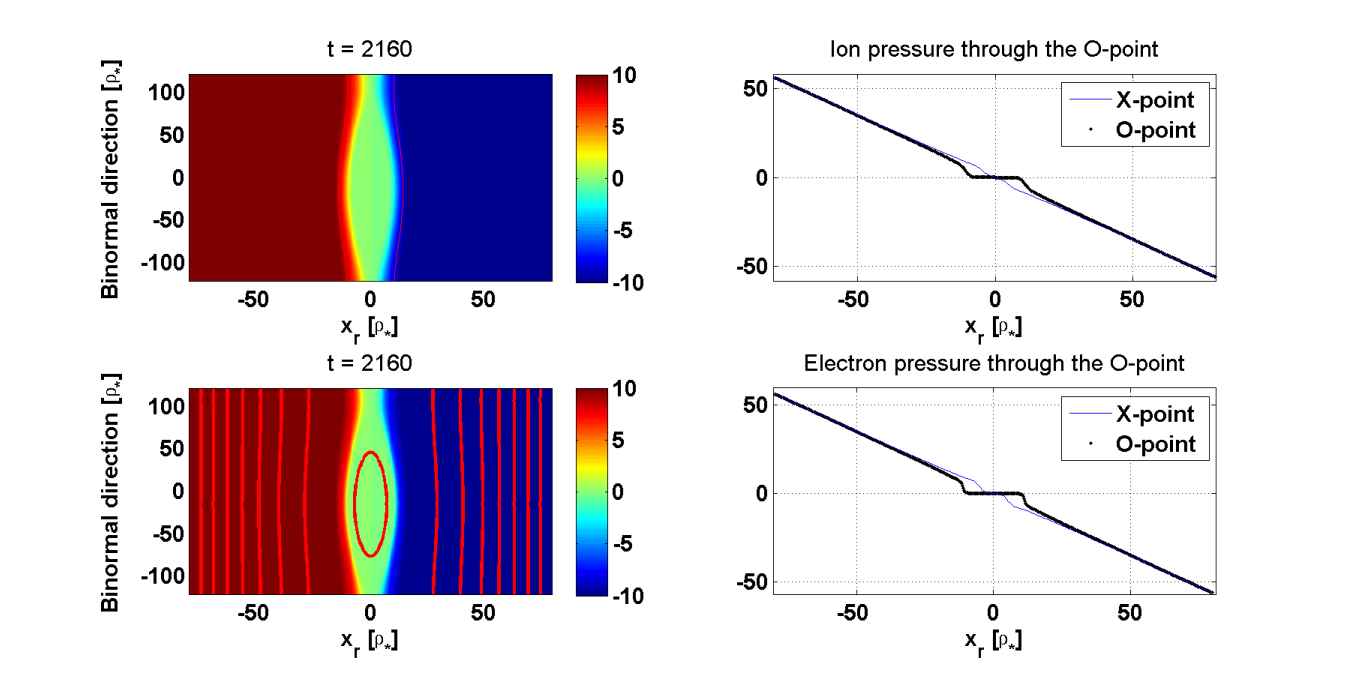
\includegraphics[width=0.7\textwidth]{pressflat.eps}
\caption{Left: 2D colormap of the pressure profiles for ions and electrons in the presence of a magnetic island. The isocontours of the vector potential are shown only with the electron colormap. Right: radial profiles of the pressure through the O (black line) and X (blue line) points.}
\label{fig:pressureflat}
\end{center}
\end{figure}

The total pressure gradient (background plus perturbed pressure) reads
\begin{equation}
{R_{\rm ref} \over L_{p_{\rm eq}+\tilde{p}}}  =  -{1 \over n_{R_0,s}T_s} {\partial (p_{s,\rm eq}+\tilde{p}_s) \over \partial \psi} = -{\partial\over\partial x_r}{\Delta p_{N,s} \over \rho_*} = 
 -{2\over 3}{\partial\tilde E_{N,s}\over\partial x_r} + {R_{\rm ref} \over L_{n,s}} + {R_{\rm ref} \over L_{T,s}}
\end{equation}

\section{Frozen electrons}

Due to the small inertia of electrons, they are considered as frozen particles to the magnetic field lines. This means in particular that the rotation frequency of electrons must equal the rotation
frequency of the island, namely
\begin{equation}
\omega_{\rm isl}\equiv\omega_{\rm TOT,e} = \omega_{*,e} + \omega_{E\times B}
\end{equation}
which constitutes the second benchmark after implementation of a magnetic island.

Therefore, the electric field must always compensate for the difference between the diamagnetic drift produced by any pressure gradient inside the island and the rotation of the island itself. In particular,
if the island does not rotate, for a sufficiently large island resulting in a complete flattening, the electrostatic potential must vanish inside the island. To verify the previous identity, one must
 conveniently quantify from the GKW outputs the diamagnetic frequency resulting from the total pressure profile and the $E\times B$ frequency.
These two quantities are derived hereafter assuming a slab geometry and considering that the binormal (in the $y$ direction) structure is determined by the island. The diamagnetic frequency in the $y$ direction reads
\begin{equation}
\omega_{*,s} = k_y{{\mathbf{b}\times\nabla p_s}\over{e_sn_sB}}\cdot\mathbf{e}_y\approx k_y{1\over{e_sn_{s,\rm eq}B}}{\partial p_s\over{\partial r}}
\end{equation}

Using the normalizations of GKW, we can write
\begin{equation}
\omega_{*,s} \approx k_y{1\over{e_{N,s}en_{R_0,s}B_NB_{\rm ref}}}{{n_{R_0,s}T_s\rho_*}\over{\rho_{\rm ref}}}{\partial\over{\partial x_r}}{\Delta p_{N,s} \over \rho_*}
\end{equation}

The temperature $T_s$ can now be expressed in terms of $T_{\rm ref}$ and $T_{R,s}$ and the reference Larmor radius used to write
\begin{equation}
\omega_{*,s} \approx k_y{1\over 2}v_{\rm th,ref}{T_{R,s}\over e_{N,s}B_N}\rho_*\left({2\over 3}{\partial\tilde E_{N,s}\over\partial x_r} - {R_{\rm ref} \over L_{n,s}} - {R_{\rm ref} \over L_{T,s}}\right)
\end{equation}

Under the assumption that the $y$ structure is determined by the island, one can write the wave number is that direction as $k_y=\pi/y_{\rm max}$, where $y_{\rm max}$ is the maximum value of the $y$ coordinate. Expressing $\rho_*$ as $\rho_*=\rho_{\rm ref}/R_{\rm ref}$ and normalizing the diamagnetic frequency to the transit frequency $\omega_t = v_{\rm th,ref}/R_{\rm ref}$ one gets the normalized diamagnetic frequency in slab geometry
\begin{equation}
\omega_{*,N,s} \approx {\pi\over y_{\rm max,N}}{1\over 2}{T_{R,s}\over e_{N,s}B_N}\left({2\over 3}{\partial\tilde E_{N,s}\over\partial x_r} - {R_{\rm ref} \over L_{n,s}} - {R_{\rm ref} \over L_{T,s}}\right)
\end{equation}

In a similar way, one can show that the $E\times B$ frequency in GKW units reads
\begin{equation}
\omega_{E,N,s} \approx {\pi\over y_{\rm max,N}}{1\over 2}{1\over B_N}{\partial\phi_{N}\over\partial x_r}
\end{equation}

Figure \ref{fig:freqsmatching} represents the profiles of the frequency for each species in the presence of an island rotating in the ion diamagnetic direction with a frequency $\omega_{\rm isl} = -0.006$. This frequency is represented by a solid black line, which must overlap the solid green line, corresponding to the total frequency of electrons. We observe this overlap everywhere inside the separatrix, but not around the X-point.

\begin{figure}
\begin{center}
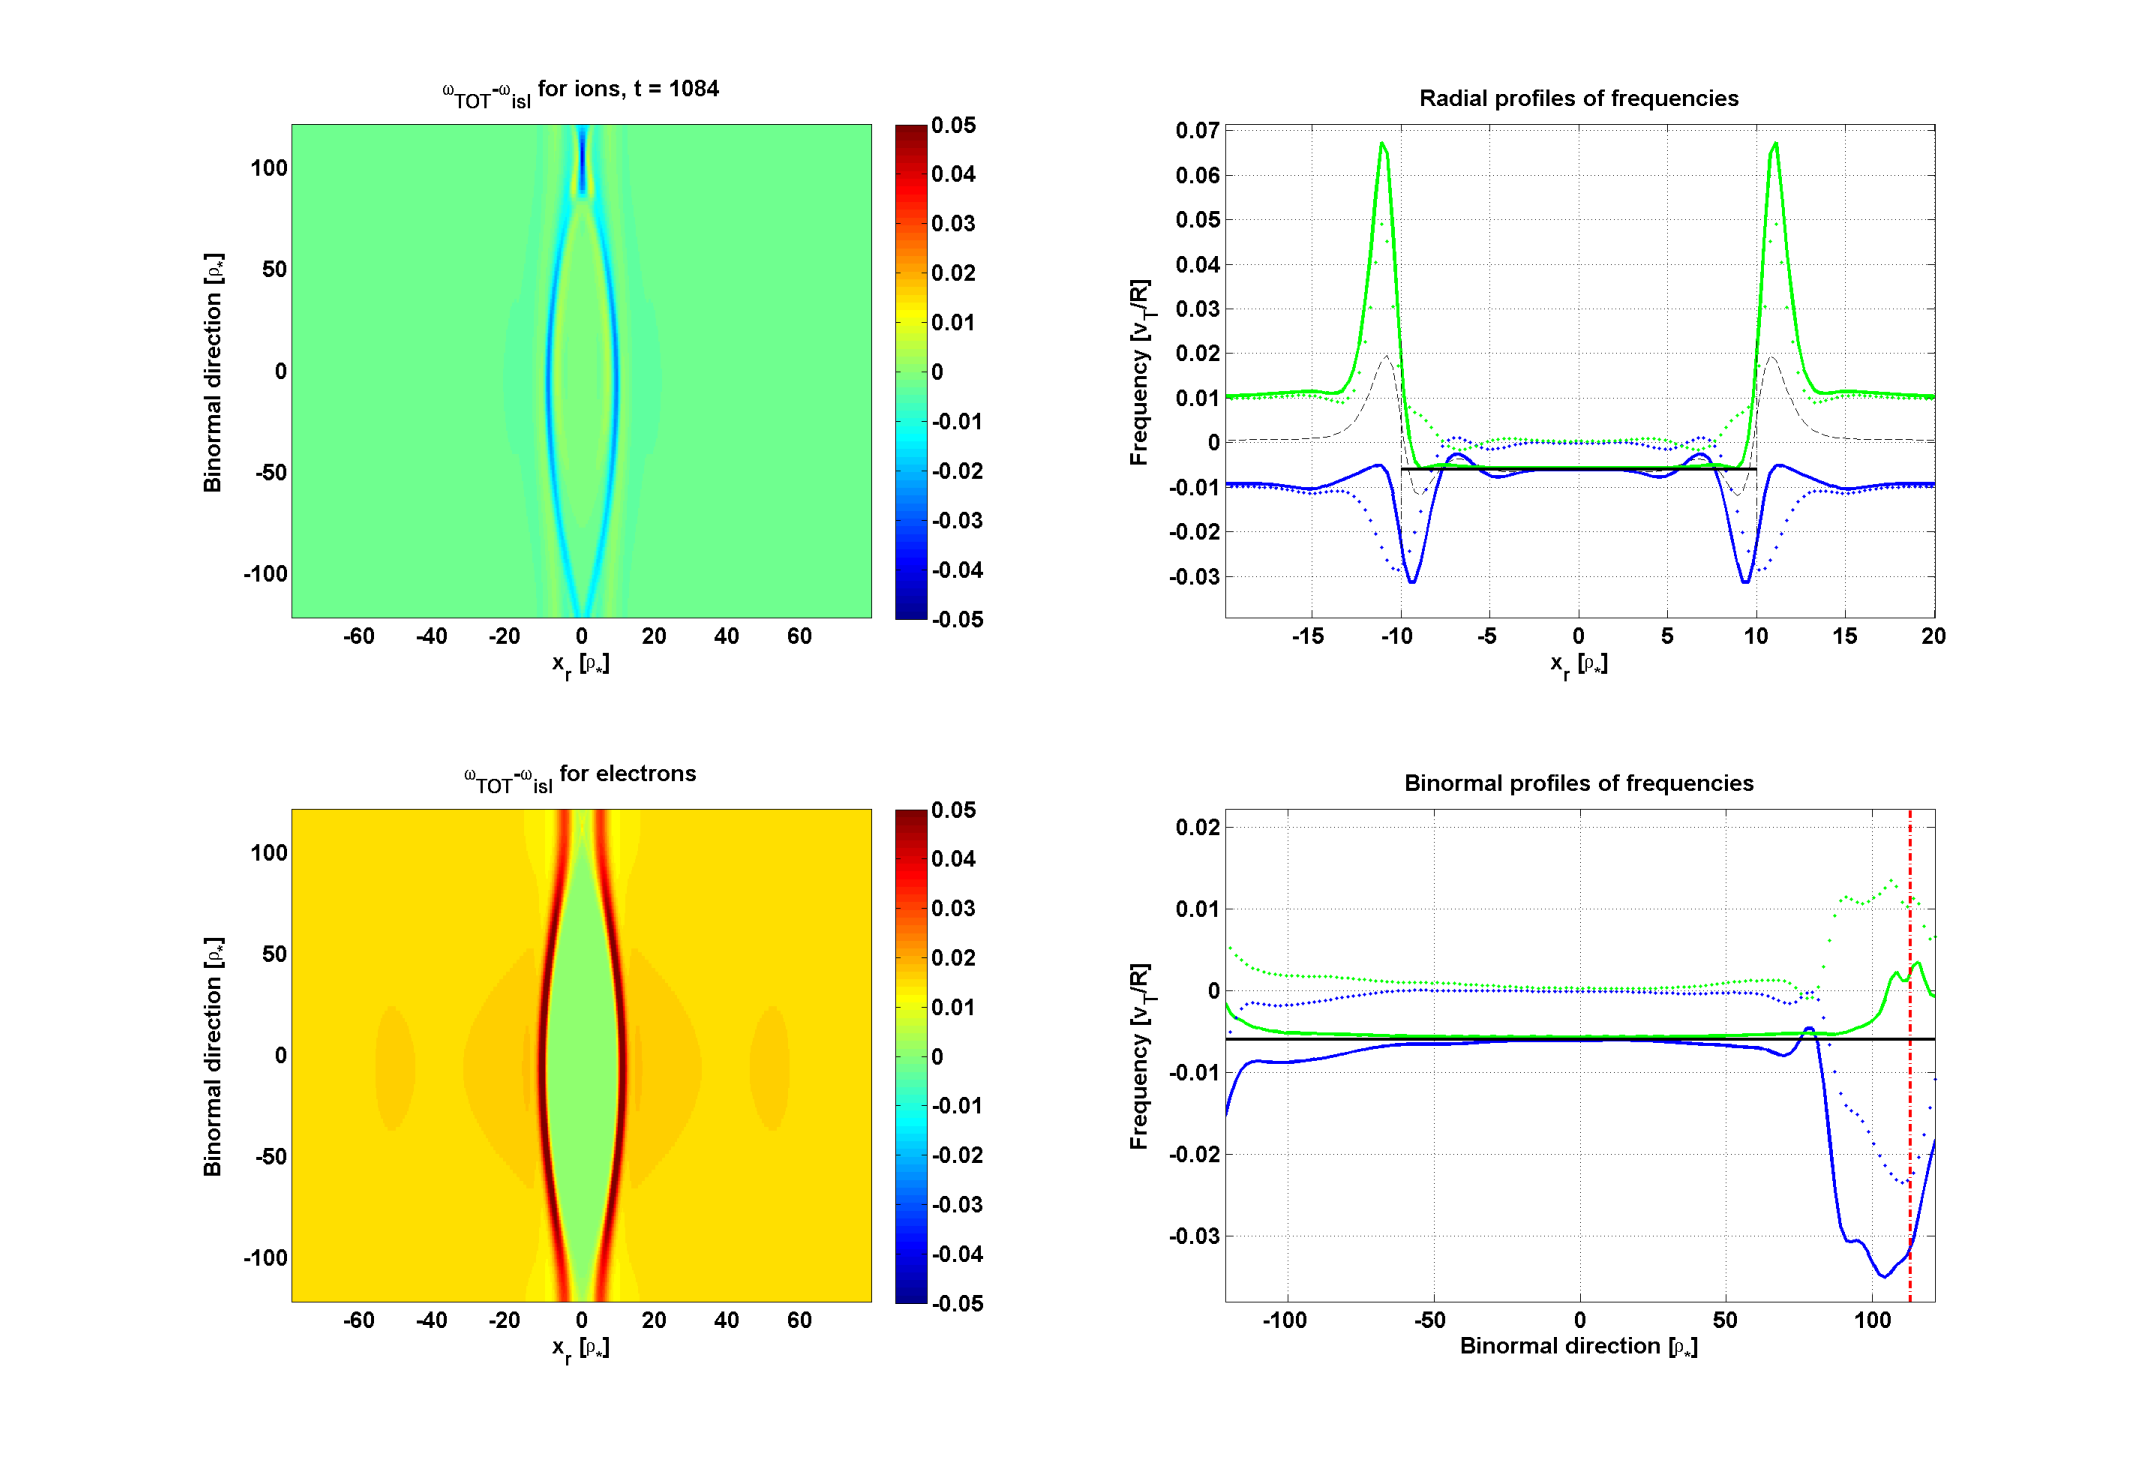
\includegraphics[width=0.7\textwidth]{freqsmatching.eps}
\caption{Left: 2D colormap of the frequency profiles for ions (up) and electrons (down) in the presence of a magnetic island with $R/L_n=0.7$ and $R/L_T=0$. Right: radial profiles of the frequency through the O-point (up) and binormal profiles of the frequency through the O and X points (down). Electrons are represented by green curves and ions by blue curves. The dotted lines represent the diamagnetic frequency and the solid lines the total frequency. For the radial profiles, the black dashed line represents the $E\times B$ frequency and the solid black line the rotation frequency of the island. For the binormal profiles, the dashed red line indicates the position of the X-point and the solid black line the rotation frequency of the island.}
\label{fig:freqsmatching}
\end{center}
\end{figure}

\section{Dependence of the electrostatic potential on the island rotation frequency}

The third and last benchmark needed after the implementation of a magnetic island constitutes the dependence of the electrostatic potential on the island rotation frequency. This dependence is calculated assuming that
 electrons inside the island short out any variation of the parallel electric field, i.e. we need to verify that $\nabla_\parallel\phi=-c^{-1}\partial_t \psi$ inside the island.
  For this we need to write an explicit expression for the parallel gradient, which is $\nabla_\parallel = \mathbf{b}\cdot\nabla$, where $\mathbf{b}=B^{-1}\mathbf{B}$ is the unit vector in the direction of the magnetic field.
  Let us perform the calculation, for the sake of simplicity, in sheared 2D slab geometry, where the magnetic field reads
  \begin{equation}
  \mathbf{B} = B_z\nabla z - \nabla\psi\times\nabla z = B_z\nabla z + {B_z x \over L_s}\nabla y - \tilde\psi k_y\sin\left(k_yy-\omega_{\rm isl}t\right)\nabla x
  \end{equation}

Under the assumption that the amplitude of the magnetic field is not significantly modified by the presence of the magnetic island and considering no derivatives in the $z$-direction (slab model), we can write
\begin{equation}
\nabla_\parallel = - {\tilde\psi k_y\over B_z}\sin\left(k_yy-\omega_{\rm isl}t\right)\partial_x + {x \over L_s}\partial_y
\end{equation}

The equation for the electrostatic potential is written as
\begin{equation}
{\tilde\psi k_y\over B_z}\sin\left(k_yy-\omega_{\rm isl}t\right){\partial\phi\over\partial x} - {x \over L_s}{\partial\phi\over\partial y} = {1\over c}{\partial \psi\over\partial t}
\end{equation}

Noticing that $x$ and $y$ coordinates must be related to each other on a flux surface for a given time $t$ by the flux label
\begin{equation}
\Omega = {x^2B_z \over 2\tilde\psi L_s} - \cos\left(k_yy-\omega_{\rm isl}t\right)
\end{equation}
we can rewrite the equation satisfied by the electrostatic potential as follows
\begin{equation}
- {x \over L_s}{\partial\phi\over\partial y} = {1\over c}{\partial \psi\over\partial t},\,\,\,\,\,{\rm for}\,\,d\Omega=0
\end{equation}
or equivalently
\begin{equation}
- {x \over L_s}\left.{\partial\phi\over\partial y}\right\vert_{\Omega} = {1\over c}{\partial \psi\over\partial t}
\end{equation}
The derivative of $x$ with respect to $y$, for $x\ne 0$, reads
\begin{equation}
{dx\over dy} = -{\tilde\psi L_s\over B_z x}\sin\left(k_yy-\omega_{\rm isl}t\right)
\end{equation}
and therefore, the equation satisfied by the electrostatic potential becomes, for $k_yy\not\equiv_\pi\omega_{\rm isl}t$
\begin{equation}
{k_y\over B_z}\left.{\partial\phi\over\partial x}\right\vert_{\Omega} = {\omega_{\rm isl}\over c}
\end{equation}
which gives, after integration
\begin{equation}
\phi = {\omega_{\rm isl}B_z\over k_y c}\left(x-h\left(\Omega\right)\right)
\end{equation}
where $h\left(\Omega\right)$ is a constant of integration for each flux surface. Note that the expression we have obtained for the electrostatic potential is only valid for $x\ne 0$ and $k_yy\not\equiv_\pi\omega_{\rm isl}t$. The function $h\left(\Omega\right)$ usually vanishes inside the island, corresponding to a complete flattening of radial profiles. Therefore, inside the separatrix and for $x\ne 0$ we can write, in GKW units
\begin{equation}
\phi_N = 2{\omega_{\rm isl,N}y_{\rm max,N}\over \pi}\Delta x_r
\end{equation}
where $\Delta x_r$ is the distance to the resonant surface. The extension to $x=0$ and $k_yy\equiv_\pi\omega_{\rm isl}t$ can be done by assuming that the electrostatic potential is continuous. Therefore, $\phi(x=0)=\lim_{x\rightarrow 0^\pm}\phi = 0$, $\phi(x=w,k_yy\equiv_\pi\omega_{\rm isl}t)=\lim_{x\rightarrow w^+}\phi = 2{\omega_{\rm isl,N}y_{\rm max,N}\over \pi}w$ and $\phi(x=-w,k_yy\equiv_\pi\omega_{\rm isl}t)=\lim_{x\rightarrow -w^-}\phi = -2{\omega_{\rm isl,N}y_{\rm max,N}\over \pi}w$. The left panel of figure \ref{fig:phiseparatrix} shows a remarkable agreement between the expected values for the electrostatic potential at the separatrix ($\Delta x_r = w$)
 from the previous expression (solid black line) and the values obtained from five simulations with GKW (red asterisks). These simulations have been performed with $w=10$, $y_{\rm max,N}=121.565$ and flat profiles.
\begin{figure}
\begin{center}
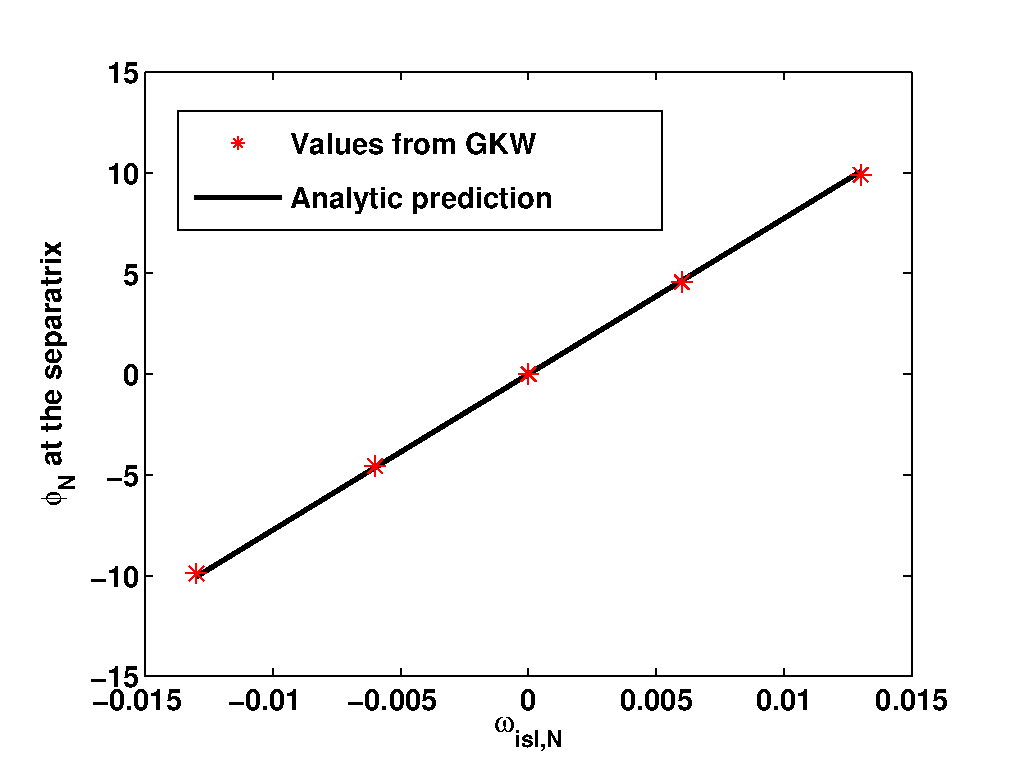
\includegraphics[width=0.4\textwidth]{phiseparatrix.eps}
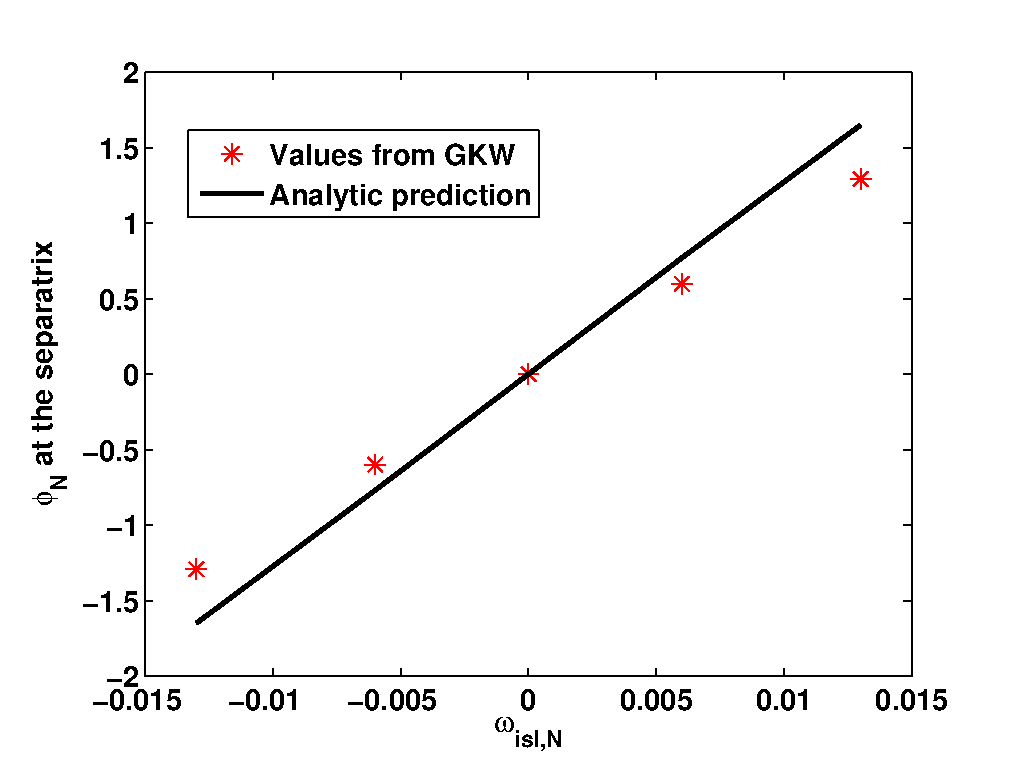
\includegraphics[width=0.4\textwidth]{phiseparatrixw2.eps}
\label{fig:phiseparatrix}
\caption{Expected values of the electrostatic potential at the separatrix (solid black line) and values obtained from simulations with GKW (red asterisks). Left: $w=10$. Right: $w=2$}
\end{center}
\end{figure}

When the island width is comparable to or smaller than the ion Larmor radius, the ion pressure profile is little modified, whereas the electron pressure profile inside the island can still be modified.
 Of course, in the absence of background density and temperature profiles, this means that the ion pressure remains almost flat, whereas the electron pressure is only modified around the separatrix. However, this
  modification is of the order of the ion Larmor radius, meaning that for an island width of the order of the ion Larmor radius the electron pressure profile will be modified inside the island.
   In this case, the equation satisfied by the electrostatic potential should include the term related to the parallel gradient of the electrons pressure inside the island, namely
\begin{equation}
\nabla_\parallel\phi=-c^{-1}\partial_t \psi + {1\over en_e}\nabla_\parallel p_e
\end{equation}

Integrating this equation leads straightforwardly to the expression
\begin{equation}
\phi = {\omega_{\rm isl}B_z\over k_y c}\left(x-h\left(\Omega\right)\right) + {1\over en_e}p_e
\end{equation}
or equivalently, in GKW units
\begin{equation}
\phi_{N,\rm sep} = 2{\omega_{\rm isl,N}y_{\rm max,N}\over \pi}w + \left.{\Delta p_{N,s} \over \rho_*}\right\vert_{\rm sep}
\end{equation}

The right panel of figure \ref{fig:phiseparatrix} shows quite a good agreement, but some differences are observed. More analysis is needed for a complete understanding in the case of small islands.


% related to auctex mode and latex-preview-mode in Emacs:
%%% Local Variables:
%%% mode: latex
%%% TeX-master: "doc"
%%% End:
